% ----------------------------------------------------------
\chapter{Arquitetura do sistema}\label{cap:arquitetura}
% ----------------------------------------------------------
 
Este capítulo delineia a arquitetura do sistema proposto, fornecendo justificativas para as decisões arquitetônicas tomadas. A proposta em questão visa desenvolver uma alternativa inovadora para a automação de pagamentos, incorporando tecnologias contemporâneas e princípios da Web 3.0, como \textit{tokens} e criptografia de dados. Elementos como a computação em nuvem, a Internet das Coisas (\gls{IoT}) e o uso de \textit{tokens} únicos, como JWT e UUID, são integrados com o objetivo de estabelecer uma infraestrutura eficaz e segura.

O sistema é composto por três componentes principais: uma aplicação \textit{web fullstack}, um servidor de \textit{sockets} e um agente de distribuição. Esses componentes interagem entre si para fornecer a funcionalidade desejada. A Figura \ref{fig:system_architecture} ilustra a arquitetura do sistema.

\begin{figure}[h]
\centering
\caption{Arquitetura do Sistema.}
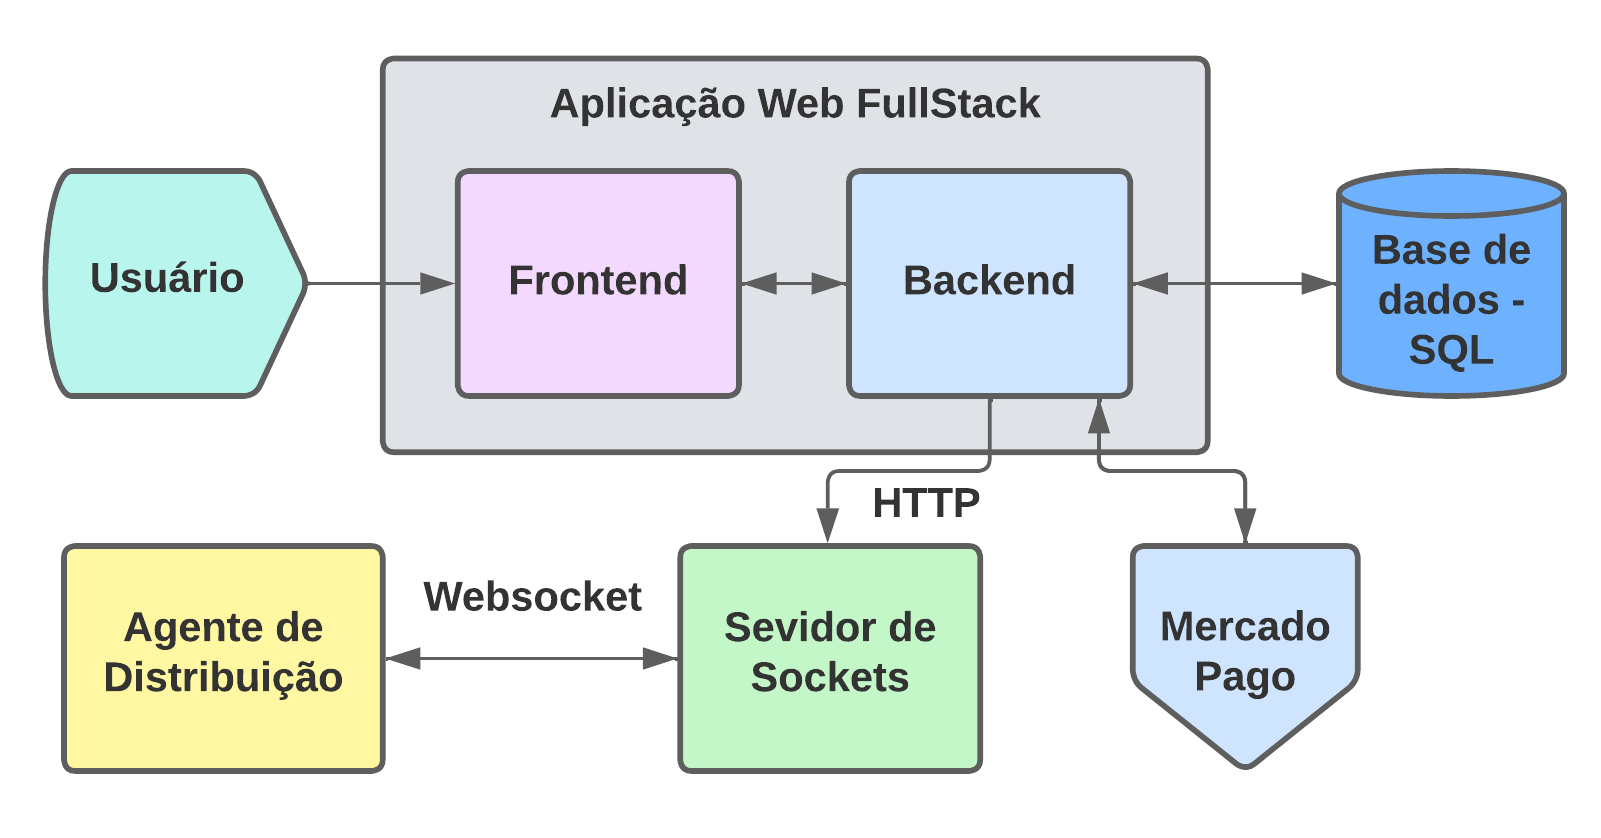
\includegraphics[width=1\textwidth]{figuras/Arquitetura.png}
\fonte{Criado pelo autor.}
\label{fig:system_architecture}
\end{figure}

Cada componente tem um papel específico no sistema e trabalha em conjunto com os outros para fornecer a funcionalidade desejada. A arquitetura foi projetada para ser escalável e eficiente, e alcança através de múltiplos meios. A implementação de \textit{sockets} em um servidor separado, evita a necessidade de \textit{pooling}, reduzindo o número de requisições ao servidor e a separação de componentes, como o banco de dados e servidor de \textit{sockets}, permite que sejam escalados separadamente para atender as demandas.

As seções 3.1 a 3.5 detalham cada um dos elementos da arquitetura. 

\section{Aplicação Web FullStack}
Este elemento é o centro do sistema e coordena todos os demais. Está dividido entre \textit{frontend} e \textit{backend} para melhor representar suas funcionalidades, porém é representado de forma única pois é dessa forma que se dá sua implementação e desenvolvimento.

\begin{enumerate}

\item \textbf{Frontend:} Esta é a interface do sistema, que é executada no dispositivo do usuário, onde o mesmo pode interagir com as lojas online cadastradas no sistema. Além disso, permite a criação, edição, visualização e exclusão de contas de administradores, lojas, itens e pedidos. É através desta interface que todas as interações do usuário com o sistema ocorrem. Estas ações serão efetuadas através de requisições para o \textit{backend} que é executado no servidor.
\item \textbf{Backend:} Esta é a \gls{API} que processa as solicitações vindas do \textit{frontend}. É neste elemento que a conexão com o banco de dados é estabelecida para recuperar e armazenar informações. Além disso, o \textit{backend} é responsável por se comunicar com a API do Mercado Pago para registrar pedidos e receber os links que permitem aos usuários efetuar pagamentos. Este componente também se conecta com a API do sistema responsável pelo gerenciamento dos \textit{websockets}, garantindo que as notificações sejam enviadas sempre que o status de um pedido for atualizado.
\end{enumerate}

\section{Servidor de Sockets}

A decisão de utilizar \textit{sockets} foi tomada para permitir que os Agentes de Distribuição recebam informações de maneira contínua. A adoção dessa tecnologia resulta em uma redução significativa no número de requisições ao servidor, especialmente quando comparada à comunicação via múltiplas requisições HTTP feitas por diversos dispositivos em intervalos curtos de tempo.

A separação deste componente da aplicação \textit{fullstack} é necessária devido às características das conexões \textit{socket}. Este tipo de conexão mantém uma comunicação contínua, o que gera uma complexidade maior tanto no desenvolvimento quanto na implantação, se comparada a uma API do tipo REST. Isso ocorre pois, para implementar \textit{sockets}, o servidor deve manter as conexões ativas indeterminadamente, algo que não é garantido por todos os provedores de hospedagem em nuvem e também não é indicado para uso na API da aplicação \textit{fullstack}, com NextJS. Este tipo de API não foi projetada para manter conexões ativas por longos períodos de tempo, e por mais que possam estabelecer conexões \textit{sockets}, isto não é uma prática recomendada em sua documentação e pelos criadores. Por esses motivos, optou-se por criar este elemento separadamente.

Este componente da arquitetura é um servidor independente, que hospeda uma API capaz de receber comunicações HTTP e  \textit{websocket}. Esta \gls{API} estabelece conexões \textit{socket} com os microcontroladores e as mantém ativas enquanto houver algum dispositivo conectado. Para garantir a segurança, as conexões devem ser autenticadas com uma chave \gls{UUID} incluída no cabeçalho de cada requisição. Além disso, cada \textit{socket} possui um ID único, permitindo a distinção entre diferentes pontos de venda.

\section{Agente de Distribuição}

Os agentes de distribuição são dispositivos que estabelecem conexão com o servidor de \textit{sockets} para receber informações e responder aos pedidos. No contexto deste trabalho, a ênfase será dada à conexão e ao recebimento de dados provenientes da API.

A implementação destes agentes de distribuição, capazes de entregar um produto ou realizar alguma tarefa paga através do sistema pode variar significativamente e não será o foco deste trabalho. Estes dispositivos incluem mas não se limitam á: aplicativos, microcontroladores, dispensers, entregadores ou uma tela que apresente os itens pedidos a uma equipe de funcionários. Portanto, a principal preocupação aqui é garantir uma comunicação eficaz e segura entre um agente de distribuição e o servidor de sockets.

\section{Mercado Pago}
Esta é a aplicação externa utilizada para efetivar os pagamentos, tem \textit{frontend e backend}. O \textit{frontend} permite ao usuário fornecer os dados de pagamento e o \textit{backend} recebe os pedidos e envia notificações. Poderia ser substituída por outra API similar, porém seriam necessárias alterações significativas na estrutura do projeto, visto que APIs diferentes utilizam métodos de autenticação e estruturas de dados diferentes.

Quando um pedido é gerado no \textit{frontend} da aplicação \textit{web}, uma requisição é feita para a API do Mercado Pago contendo informações deste pedido e um token do sistema. Ao receber estas informações do pedido, a API retorna um link contendo o endereço de uma página onde o usuário pode realizar o pagamento. Assim que o pagamento é confirmado internamente pelo Mercado Pago, a API envia uma notificação para o \textit{backend} da aplicação web deste sistema, informando que houve uma atualização no pedido, e a aplicação web faz uma nova requisição para a API do Mercado Pago, para obter o status do pedido atualizado.

\section{Base de Dados}

É o banco de dados da aplicação, deve ser capaz de armazenar itens, pedidos, usuários, pontos de vendas e quaisquer outros elementos necessários ao sistema.

%---------------------------------------------------------------------------------------
\chapter{Implementação}\label{cap:desenvolvimento}
%---------------------------------------------------------------------------------------

Este capítulo descreve o desenvolvimento do projeto, que envolveu a aplicação dos conceitos apresentados na fase de fundamentação teórica e a aplicação da arquitetura definida. O capítulo é dividido em quatro seções: a Seção \ref{cap:bancodedados} fala sobre o banco de dados, a Seção \ref{cap:fullstack} apresenta a aplicação \textit{web full-stack}, a Seção \ref{cap:sockets} traz a definição o servidor de \textit{sockets} e a Seção \ref{cap:agent} aborda o agente de distribuição.

\section{Banco de Dados} \label{cap:bancodedados}

A primeira etapa do processo de desenvolvimento foi a modelagem do banco de dados relacional. O modelo definido é composto por quatro entidades fundamentais: usuários, pontos de venda (PDVs), pedidos e itens. Cada entidade possui seus atributos específicos e suas relações com as outras entidades. O \glsxtrfull{ERD} do banco de dados, obtido através da ferramenta DBeaver está representado pela Figura \ref{fig:database}. A seguir são descritas cada uma das entidades presentes na Figura \ref{fig:database}:

\begin{figure}
	\caption{\label{fig:database}ERD - Projeto.}
	\begin{center}
		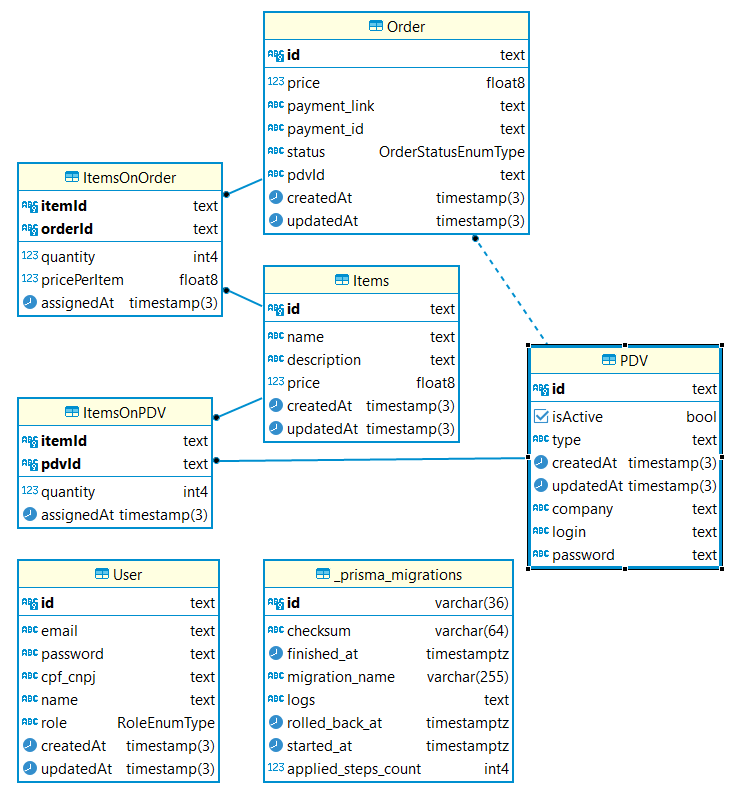
\includegraphics{figuras/database.png}
	\end{center}
	\fonte{Criado pelo autor.}
\end{figure}

\begin{itemize}
    \item \textit{User} (Usuário): Este modelo representa um usuário do sistema. Os usuários têm uma identificação única (id), e-mail, senha, cpf/cnpj, nome, cargo (role), além dos campos de controle createdAt e updatedAt.
    \item RoleEnumType: Este é um tipo de enumeração que define os possíveis papéis que um usuário pode ter: user (usuário) ou admin (administrador).
    \item PDV (Ponto de Venda): Representa um ponto de venda dentro do sistema. Cada PDV tem uma identificação única, estado (ativo ou não), tipo, empresa (company), login, senha e duas listas de itens e pedidos relacionados a ele.
    \item \textit{Order} (Pedido): Representa um pedido feito no sistema. Cada pedido tem uma identificação única, uma lista de itens (ItemsOnOrder), preço, link de pagamento, identificação de pagamento, status, identificação do ponto de venda onde foi feito e os campos de controle createdAt e updatedAt.
    \item OrderStatusEnumType: Este é um tipo de enumeração que define os possíveis estados que um pedido pode ter: pending (pendente), approved (aprovado), accredited (creditado), delivered (entregue), canceled (cancelado).
    \item ItemsOnOrder (Itens no Pedido): Representa a relação entre pedidos e itens. Ele inclui a quantidade de cada item no pedido, o preço por item, a identificação do item, a identificação do pedido e a data em que o item foi atribuído ao pedido.
    \item ItemsOnPDV (Itens no Ponto de Venda): Representa a relação entre os pontos de venda e os itens. Ele inclui a quantidade de cada item no ponto de venda, a identificação do item, a identificação do ponto de venda e a data em que o item foi atribuído ao ponto de venda.
    \item Items (Itens): Representa um item que pode ser vendido em um ponto de venda e incluído em um pedido. Cada item tem uma identificação única, nome, descrição, preço e listas de pedidos e pontos de venda aos quais está associado.
    \item Prisma Migrations: Este modelo é utilizado pelo ORM Prisma para controlar as alterações na estrutura do banco, controlando quais migrations foram aplicadas no banco de dados, permitindo um versionamento deste.
\end{itemize}

Em termos de relacionamentos, os usuários (User) não estão diretamente associados a outras entidades. Os pedidos (Order) estão associados a um ponto de venda (PDV) numa relação muitos pra um, através da coluna pdvId na tabela Order, e de muitos para muitos com itens (Items), através da tabela ItemsOnOrder. Já os pontos de venda (PDV) tem uma associação de um para muitos com itens através da entidade ItemsOnPDV.

Optou-se pela utilização do PostgreSQL como banco de dados, e foram incluídas as entidades citadas anteriormente, seguindo a sintaxe do Prisma de forma a criar e se comunicar com o banco de dados. O Código \ref{code:prisma} exibe a declaração da tabela User, usando a sintaxe do Prisma.

\begin{figure}[h]
\begin{lstlisting}[caption={Exemplo de um schema no Prisma.}, label={code:prisma}]
generator client {
    provider = "prisma-client-js"
}

datasource db {
    provider = "postgresql"
    url      = env("DATABASE_URL")
}

model User {
    id        String        @id @unique @default(uuid())
    email     String        
    password  String
    cpf_cnpj  String        @unique
    name      String
    role      RoleEnumType? @default(user)
    createdAt DateTime      @default(now())
    updatedAt DateTime      @updatedAt
}

enum RoleEnumType {
    user
    admin
}
    
\end{lstlisting}

\fonte{Criado pelo autor.}
\end{figure}

\section{Aplicação Web Full Stack} \label{cap:fullstack}

A aplicação web foi desenvolvida utilizando o \textit{framework} Next.js, que permite a criação de aplicações fullstack com React. A IDE escolhida foi o Visual Studio Code (VS Code). Como o Next.js é um \textit{framework full-stack}, tanto o \textit{front-end} quanto o \textit{back-end} foram desenvolvidos dentro de um projeto NextJS. Pode-se destacar algumas bibliotecas como o tRPC para criação das rotas da API no \textit{backend} e acesso a elas no \textit{frontend}, material UI que é uma biblioteca de componentes React de código aberto, Zod para verificação de dados e Prisma como \gls{ORM} para gerenciar o banco de dados. 

A aplicação possui três pontos de entrada para os usuários: a página para compras, a página de gestão de um ponto de vendas, e a página de gestão do sistema. A página de compras é pública, já as páginas de gestão de um ponto de vendas e gestão do sistema contam com autenticação, onde o usuário deve ter um login e senha autorizados. Cada ponto de vendas tem um acesso, conforme estabelecido no momento em que foi cadastrado, já para o acesso de gestão do sistema, múltiplos acessos podem ser cadastrados. 

\subsection{Fluxo de Compras}

A Figura \ref{fig:compra} mostra o fluxograma de compra para um cliente. Ao acessar a página de compras, o sistema segue um layout tradicional, listando todos os produtos em uma lista e exibindo para o usuário o preço total, como exibido na Figura \ref{fig:loja}. Quando o usuário finaliza a compra, é redirecionado para o pagamento através do Mercado Pago. A API do Mercado Pago foi escolhida por permitir o pagamento via PIX e por disponibilizar uma interface muito completa e confiável para o usuário, sendo uma marca conhecida no Brasil e que traz diversas garantias e verificações para o processo de pagamento.

\begin{figure}
	\caption{\label{fig:compra}Fluxograma de compra.}
	\begin{center}
		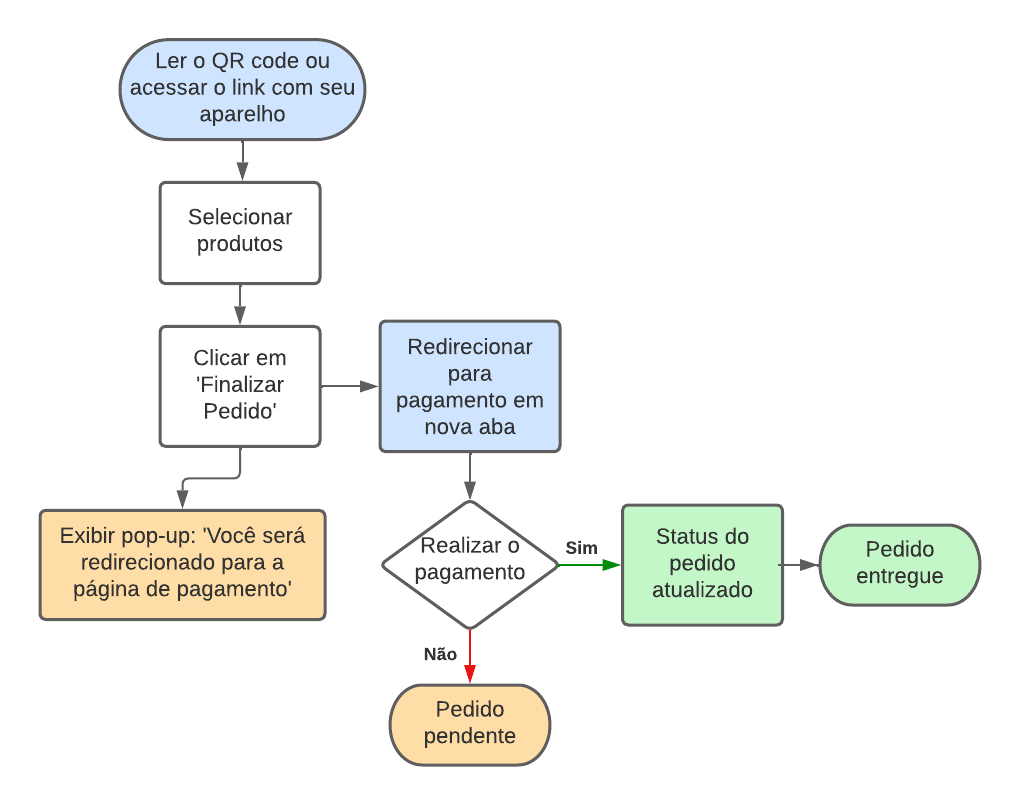
\includegraphics[width=0.8\textwidth]{figuras/Diagrama compra.png}
	\end{center}
	\fonte{Criado pelo autor.}
\end{figure}

\begin{figure}
	\caption{\label{fig:loja}Página da loja.}
	\begin{center}
		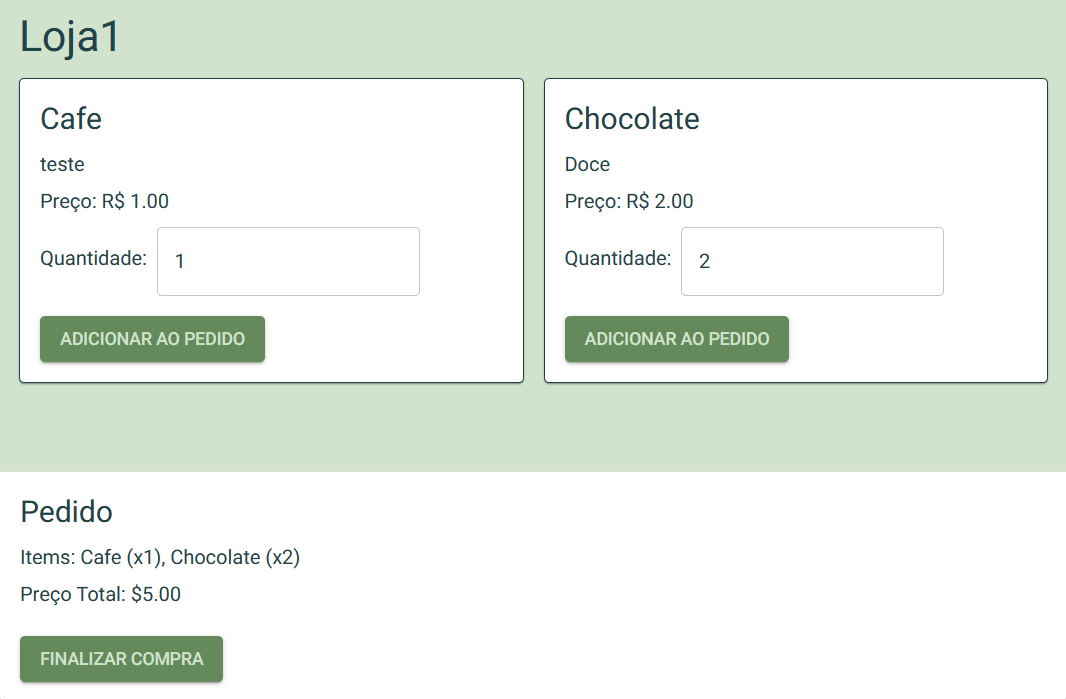
\includegraphics[width=\textwidth]{figuras/loja.png}
	\end{center}
	\fonte{Criado pelo autor.}
\end{figure}

Assim que o pagamento é efetuado, uma notificação é enviada para a API da aplicação Web, e a aplicação realiza uma requisição ao servidor do Mercado Pago para obter confirmação do pagamento.

Ao ser confirmado o pagamento, a aplicação Web envia uma requisição HTTP Post para a API que controla os Websockets, de forma a postar uma mensagem na conexão do ponto de vendas em que ocorreu a compra.

\subsection{Fluxo de Administração do Sistema}

A administração do sistema, apenas pode ser feita por usuários autorizados através da página de \textit{login}. Um administrador pode visualizar, criar, editar e excluir pontos de vendas e usuários administradores. Além disso, contas de administrador têm acesso à página ``log de pagamentos'',  que exibe as últimas notificações recebidas da API do Mercado Pago. A Figura \ref{fig:admin} representa o diagrama de administração do sistema.

\begin{figure}
	\caption{\label{fig:admin}Fluxograma administrativo.}
	\begin{center}
		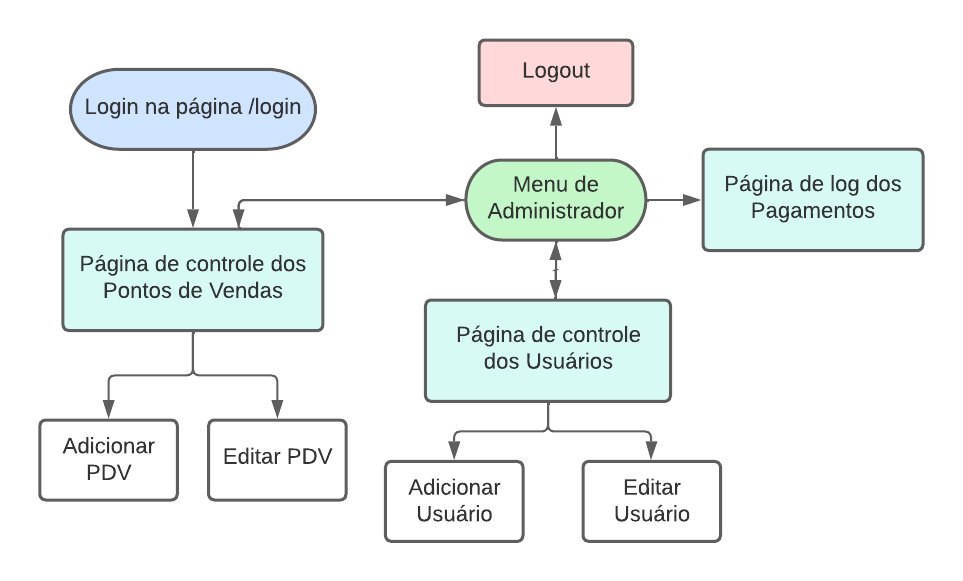
\includegraphics[width=0.8\textwidth]{figuras/Diagrama administrativo.png}
	\end{center}
	\fonte{Criado pelo autor.}
\end{figure}

\subsection{Fluxo de Administração de Um Ponto de Vendas}

O controle de um ponto de vendas apenas pode ser acessado através da página de \textit{login} para controle de loja. A Figura \ref{fig:pdv} mostra um fluxograma com as opções para controle de um ponto de vendas. Através desse acesso o usuário pode visualizar, criar, editar e excluir itens de um ponto de venda, gerenciar e visualizar pedidos, e também pode acessar a página da loja ligada ao ponto de vendas, para conferir como está a interface onde os clientes realizam os pedidos. 

\begin{figure}
	\caption{\label{fig:pdv}Fluxograma do controle de um ponto de vendas.}
	\begin{center}
		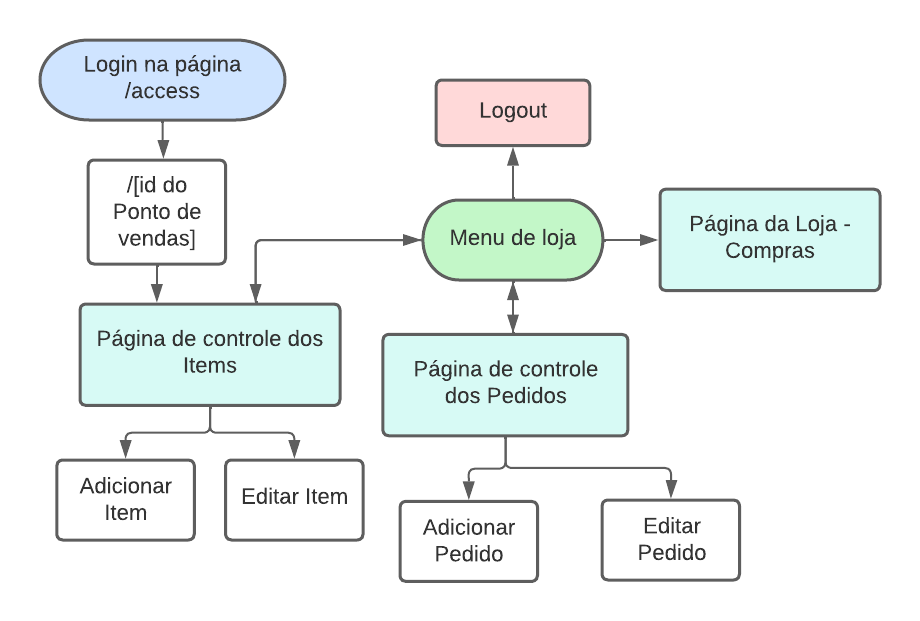
\includegraphics[width=0.8\textwidth]{figuras/Diagrama de controle de loja.png}
	\end{center}
	\fonte{Criado pelo autor.}
\end{figure}

\subsection{\textit{Frontend}}

O \textit{frontend} foi desenvolvido utilizando React, uma biblioteca JavaScript para construção de interfaces de usuário. A interface foi projetada para ser intuitiva e simples. Ela utiliza no \textit{layout} componentes da biblioteca Material UI, uma biblioteca de componentes que implementa o Material Design do Google, e componentes criados com HTML e CSS. Foram criadas páginas para a listagem, criação, edição e exclusão de usuários e pontos de venda. A Figura \ref{fig:pdvs} mostra a tela do painel do administrador que permite o controle dos pontos de vendas, e representa o layout que foi seguido ao longo de todo o frontend para listar dados.

\begin{figure}
	\caption{\label{fig:pdvs}Tela de controle de PDVs.}
	\begin{center}
		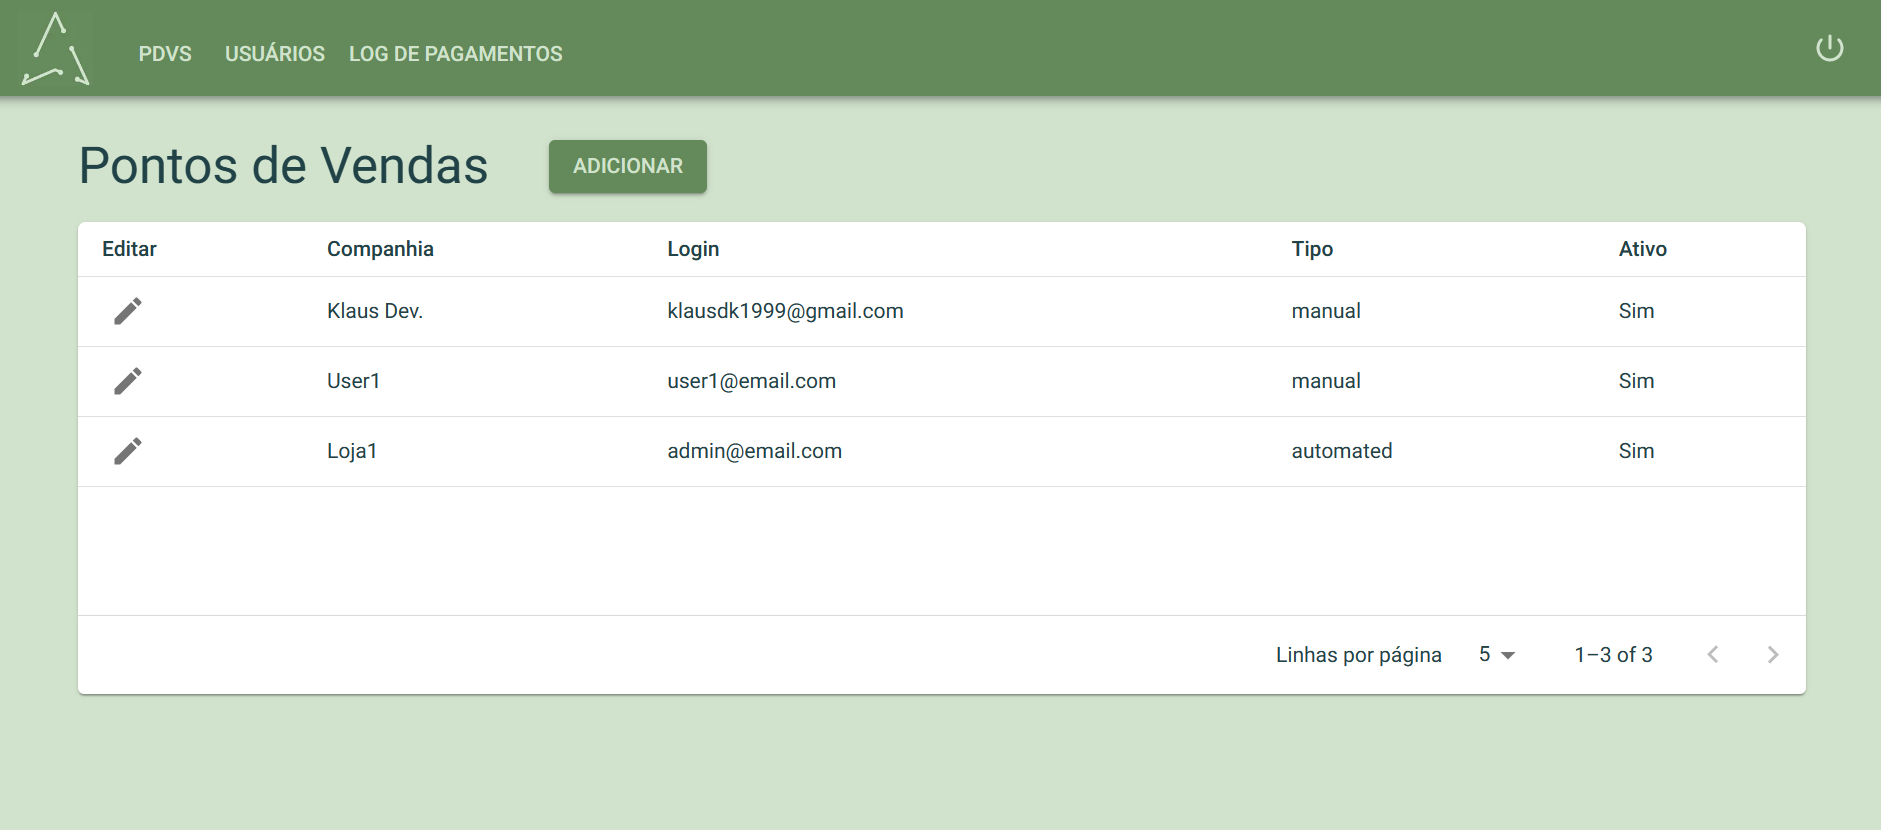
\includegraphics[width=\textwidth]{figuras/tela pontos de vendas.png}
	\end{center}
	\fonte{Criado pelo autor.}
\end{figure}

Além do \textit{layout} anterior, usado para listagem, outro \textit{layout} que aparece em vários locais do sistema destina-se a coleta de informações, representado na Figura \ref{fig:crud}, usado para adicionar e editar informações. 

\begin{figure}
	\caption{\label{fig:crud}Tela para adicionar Item.}
	\begin{center}
		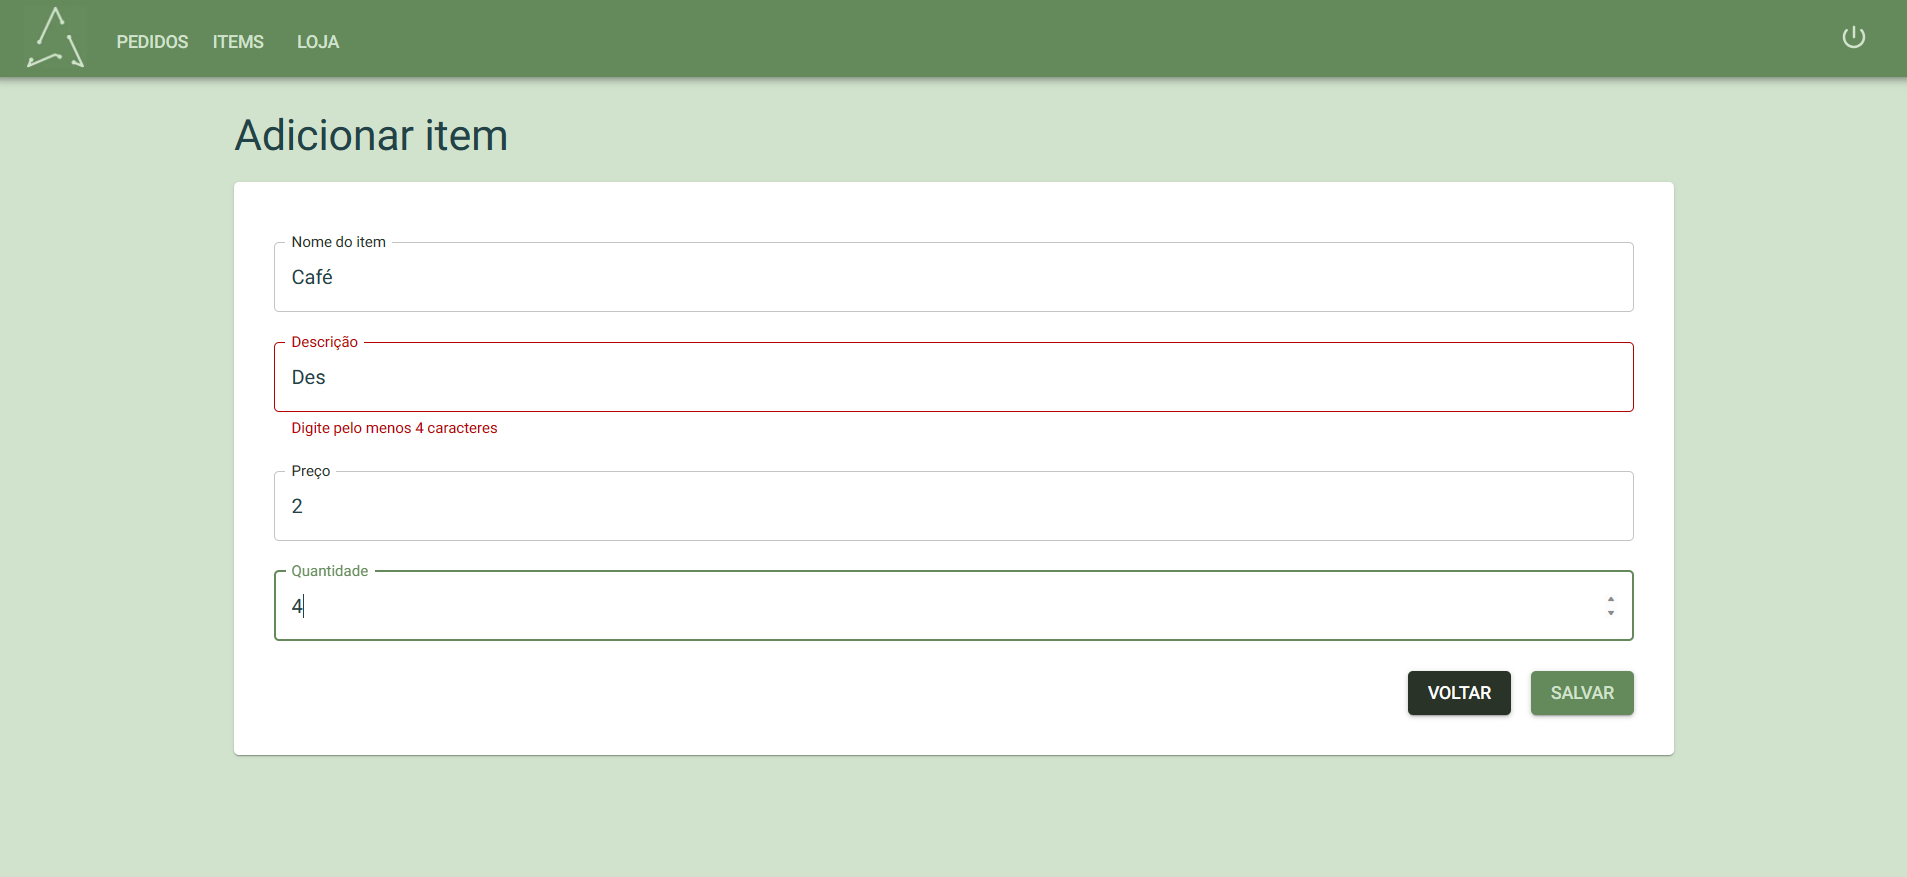
\includegraphics[width=\textwidth]{figuras/adicionar.png}
	\end{center}
	\fonte{Criado pelo autor.}
\end{figure}

\subsection{\textit{Backend}} 

A API \textit{backend} dentro da aplicação \textit{full-stack} foi dividida em grupos de rotas, acordo com as entidades do banco de dados envolvidas. Existem grupos de rotas para autenticação, itens, pedidos, pontos de vendas e usuários. Um exemplo de rota pode ser visto no Código \ref{code:prisma}. Trata-se da rota de \textit{login} que exige como entrada um objeto com os campos  ``email'' e  ``password''. Se esses parâmetros forem fornecidos corretamente, o processo descrito como \textit{mutation} é iniciado. Uma \textit{mutation} se refere a qualquer procedimento que altera o estado dos dados. Nesse caso, a ação desejada é realizada e a senha criptografada no banco é comparada com a senha recebida na rota. O Código \ref{code:login} mostra como a rota de login foi implementada e parte do processo de autenticação.

\begin{figure}[h]
\begin{lstlisting}[caption={Exemplo de uma rota tRPC.}, label={code:login}]
export const authRouter = createTRPCRouter({
  login: publicProcedure
    .input(
      z.object({
        email: z.string(),
        password: z.string().min(4),
      })
    )
    .mutation(async ({ input, ctx }) => {
      const { res } = ctx;
      const { email, password } = input;

      const databaseUser = await ctx.prisma.user.findFirst({
        where: { email: email },
      });
      if (!databaseUser) {
        throw new TRPCError({
          code: "NOT_FOUND",
          message: "Usuario nao encontrado",
        });
      }

      const isPasswordValid = bcrypt.compareSync(
        password,
        databaseUser.password
      );
\end{lstlisting}
\fonte{Criado pelo autor.}
\end{figure}

O tRPC serve como um gerenciador destas rotas. Diferente de uma API mais comum, onde o desenvolvedor especifica o caminho de cada rota, e precisa criar verificações para os tipos e respostas, o tRPC, em conjunto com o Zod, fornecem esta estrutura, cabendo ao desenvolver apenas definir quais dados devem ser recebidos, sem a necessidade de criar os meios de verificação. 

As rotas implementadas, além de serem utilizadas pelas páginas do frontend para enviar e receber dados, também fazem as conexões externas, como confirmação de pagamentos com a API do Mercado Pago e envio de mensagens para a API de Websockets.

O desenvolvimento da aplicação web resultou em um sistema funcional que atende aos requisitos estabelecidos na seção de objetivos deste trabalho. Foram criadas telas para o cadastro de usuários, pontos de venda e pedidos, além de telas para a visualização e edição dessas informações. O sistema conta com autenticação de usuários e utilização de \textit{tokens} JWT para garantir a segurança das informações.

A interface do sistema foi desenvolvida seguindo boas práticas de usabilidade e design, resultando em uma interface intuitiva e fácil de usar para os usuários finais.

\section{Servidor de \textit{Sockets}} \label{cap:sockets}
Este elemento do sistema é um servidor \textit{websocket} construído com a biblioteca Fastify para Node.js, com autenticação por chave de acesso e suporte a conexões \glsxtrfull{CORS}\footnote{CORS é um mecanismo que permite que muitos recursos (por exemplo, fontes, JavaScript, etc.) em uma página da web sejam solicitados de outro domínio fora do domínio da qual a origem da solicitação foi feita.}. Ele é encarregado da comunicação entre o servidor e os agentes de distribuição, permitindo que as atualizações sejam enviadas assim que ocorrem, sem a necessidade de solicitações constantes. Este método de comunicação foi escolhido por permitir uma melhor escalabilidade do sistema, reduzindo o número de requisições que precisam ser processadas pelo servidor.

Ao final do desenvolvimento, é possível criar conexões do tipo \textit{socket} privadas, e enviar mensagens para os \textit{sockets} via requisições HTTP, atendendo as necessidades de comunicação do sistema entre a API e os agentes de distribuição. A seguir será detalhado o funcionamento do servidor.

\subsection{Configurações iniciais e Criação do servidor \textit{websocket}}  As variáveis de ambiente são carregadas utilizando a biblioteca \texttt{dotenv} e instância do Fastify é criada, e configurada para permitir requisições de qualquer origem e para os métodos GET e POST.

Uma instância do servidor \textit{websocket} é criada usando a biblioteca \texttt{ws}. O servidor \textit{websocket} é configurado para não criar um servidor HTTP próprio, pois o servidor HTTP será fornecido pelo Fastify.

\subsection{Gerenciamento e Atualização de conexões \textit{websocket}} Uma lista para armazenar as conexões \textit{websocket} é criada. Cada conexão é identificada por uma \textit{string}, que é obtida do URL da requisição que abriu a conexão. O servidor \textit{websocket} é configurado para lidar com eventos de conexão, mensagem e fechamento. Quando uma nova conexão é estabelecida, o servidor registra a conexão em uma lista de conexões. Quando uma mensagem é recebida, o servidor a envia para a conexão a qual se destina. Quando uma conexão é fechada, o servidor remove a conexão do mapa.

O servidor Fastify é configurado para lidar com eventos de upgrade de conexões HTTP para \textit{websocket}. Quando uma requisição de upgrade é recebida, o servidor verifica se a chave de acesso fornecida nos cabeçalhos da requisição é válida. Se a chave de acesso for válida, a requisição de upgrade é passada para o servidor WebSocket. Caso contrário, a conexão é encerrada.

\subsection{Roteamento HTTP e Socket} 

Duas rotas HTTP são definidas:

\begin{itemize}
    \item \textbf{GET "/status"} - retorna uma mensagem indicando que o servidor está online.
    \item \textbf{POST "/post"} - é usada para enviar mensagens através das conexões WebSocket. Antes de tratar a requisição, a rota verifica se a chave de acesso fornecida nos cabeçalhos da requisição é válida. Se a chave de acesso for válida, a requisição é processada. A requisição deve incluir no corpo um ID de conexão e uma mensagem. A mensagem é enviada através da conexão socket correspondente ao ID fornecido.
\end{itemize}

Para conexão via WebSocket:
\begin{itemize}
    \item \textbf{ws://\{endereço do servidor\}/\{ID do socket\}} - conecta no socket com o ID passado como parâmetro. Similar a rota HTTP /post, antes de tratar a conexão, a rota verifica se a chave de acesso fornecida nos cabeçalhos da requisição é válida.
\end{itemize}

\section{Agente de distribuição} \label{cap:agent}

O desenvolvimento de um agente de distribuição se deu através de um microcontrolador NodeMCU ESP8266 e da plataforma Arduino IDE. O código do controlador desenvolvido em C++, inclui as bibliotecas ESP8266WiFi.h, que permite que o dispositivo se conecte com qualquer rede wifi, e WebSocketsClient.h que permite a conexão com \textit{websocket}. O microcontrolador se conecta no \textit{websocket}, com o UUID do ponto de vendas, e verifica cada mensagem recebida. Neste projeto a ênfase será na conexão e recebimento de dados do servidos de \textit{socket}, e o microcontrolador acende um led para demonstrar que recebeu a notificação. A Figura \ref{fig:diagrama conexao} apresenta o funcionamento do microcontrolador.

\begin{figure}
	\caption{\label{fig:diagrama conexao}Diagrama da conexão NodeMCU e servidor.}
	\begin{center}
		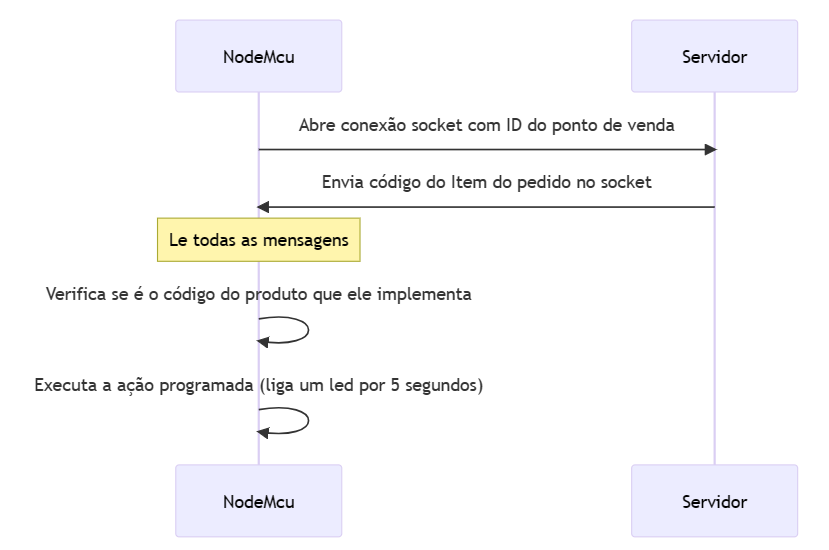
\includegraphics[width=\textwidth]{figuras/diagrama nodemcu.png}
	\end{center}
	\fonte{Criado pelo autor.}
\end{figure}

Para implementar um agente de distribuição, este deverá verificar pelos códigos de itens presentes no ponto de venda, e implementar o que for necessário para fazer a entrega de cada item.

O desenvolvimento do agente de distribuição no NodeMCU resultou em um dispositivo funcional capaz de se comunicar com a aplicação web e receber dados sobre o status dos pedidos. Foram realizados testes que provaram a integração do NodeMCU com a aplicação web e validaram o recebimento de dados sobre o status dos pedidos. Eles serão detalhados na Seção \ref{cap:host}.

Uma alternativa para este agente de distribuição automático, é a utilização da interface para controle de pedidos do ponto de vendas, exibida na Figura \ref{fig:pedidos}. Este método é chamado de ``manual'', e pode ser selecionado no momento de criação do ponto de vendas no sistema. Pontos de vendas manuais não precisam de um agente de distribuição e os pedidos devem ser atualizados manualmente. Eles não utilizam conexões no servidor de \textit{socket} e devem ser controlador inteiramente pelo usuário através da interface. O método apresentado anteriormente, com um agente de distribuição conectado via \textit{socket}, é definido como ``automated'' no momento da criação do ponto de vendas e é considerado o padrão.

\begin{figure}
    	\caption{\label{fig:pedidos}Tela de pedidos.}
    	\begin{center}
    		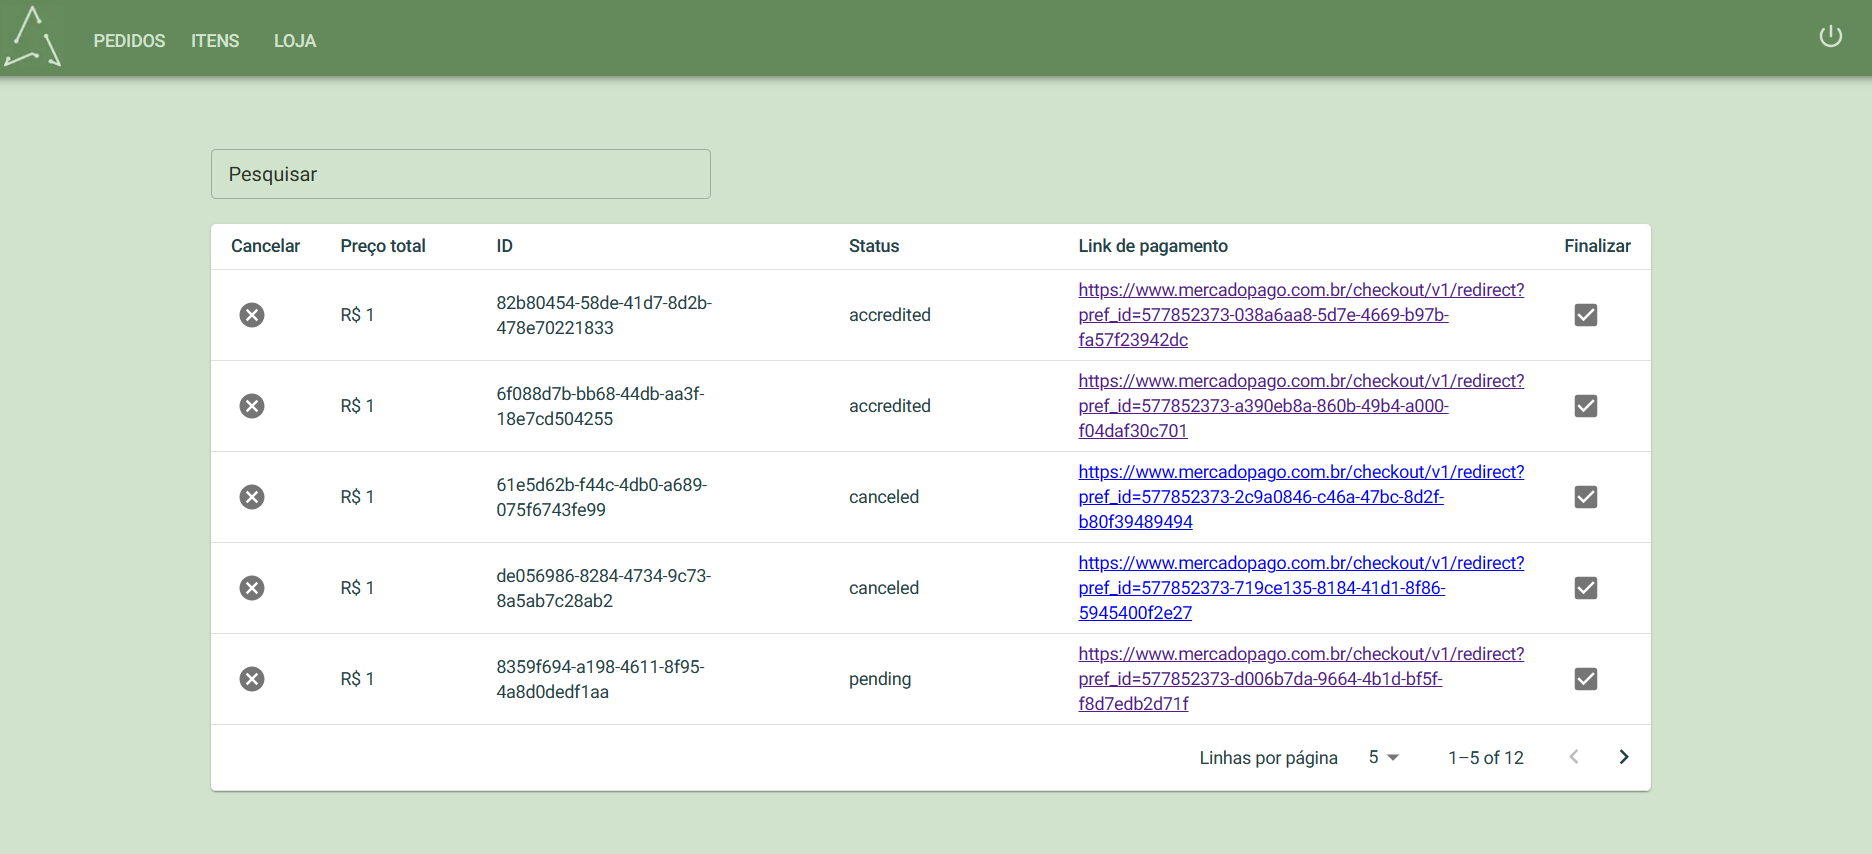
\includegraphics[width=0.8\textwidth]{figuras/pedidos.png}
    	\end{center}
    	\fonte{Criado pelo autor.}
\end{figure}

\chapter{Resultados}\label{cap:resultados}

Este capítulo apresenta os resultados alcançados com a execução e implementação do projeto. O capítulo é dividido em 3 seções: a Seção \ref{cap:test} trata dos testes de funcionamento, a Seção \ref{cap:host} trata da hospedagem e a Seção \ref{cap:final} trata das considerações finais.
    
\section{Resultados e testes da implantação em ambiente de produção} \label{cap:test}

Para testar o sistema e demonstrar na prática os resultados obtidos, será simulado o processo de compra de um café em um ponto de vendas programado para o teste. Os passos simulados são os seguintes:

\begin{itemize}
    \item Para fazer uma compra, o cliente deve acessar a página loja do ponto de venda em que deseja fazer a compra. A Figura \ref{fig:qrstore} mostra um QR code que redireciona para a loja de testes do sistema. O mesmo poderia estar presente em um ponto de vendas físico, ou o link\footnote{\url{https://quickpay.vercel.app/store/00f138a0-e8ac-4497-8eb9-057fcf2dec0d}} poderia ser fornecido ao cliente diretamente para vendas via chat virtual.


    \begin{figure}
    	\caption{\label{fig:qrstore}QR code para a loja de testes.}
    	\begin{center}
    		
\includegraphics[width=0.4\textwidth]{figuras/qrcodestore.png}
    	\end{center}
    	\fonte{Criado pelo autor.}
    \end{figure}

    \item Na loja \textit{online}, o cliente seleciona o produto que deseja e clica em ``finalizar compra''. A Figura \ref{fig:testeloja} mostra a loja de testes. Ao clicar em finalizar compra uma mensagem é exibida, indicando ao usuário a página de pagamentos, Figura \ref{fig:avisopagamento}.

    \begin{figure}
    	\caption{\label{fig:testeloja}Loja de testes.}
    	\begin{center}
    		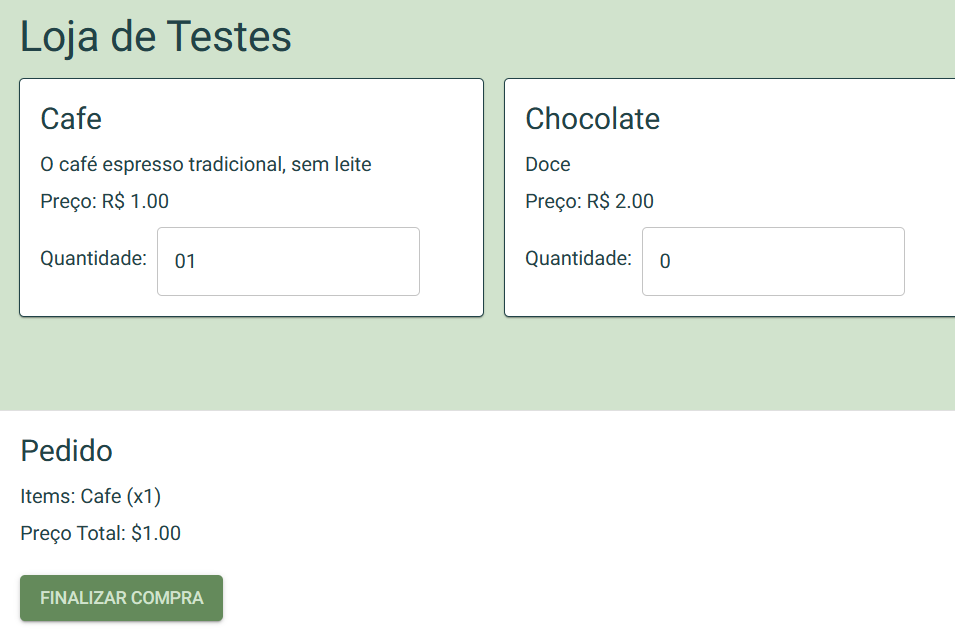
\includegraphics[width=0.8\textwidth]{figuras/testeloja.png}
    	\end{center}
    	\fonte{Criado pelo autor.}
    \end{figure}

    \begin{figure}
    	\caption{\label{fig:avisopagamento}Mensagem ao finalizar compra.}
    	\begin{center}
    		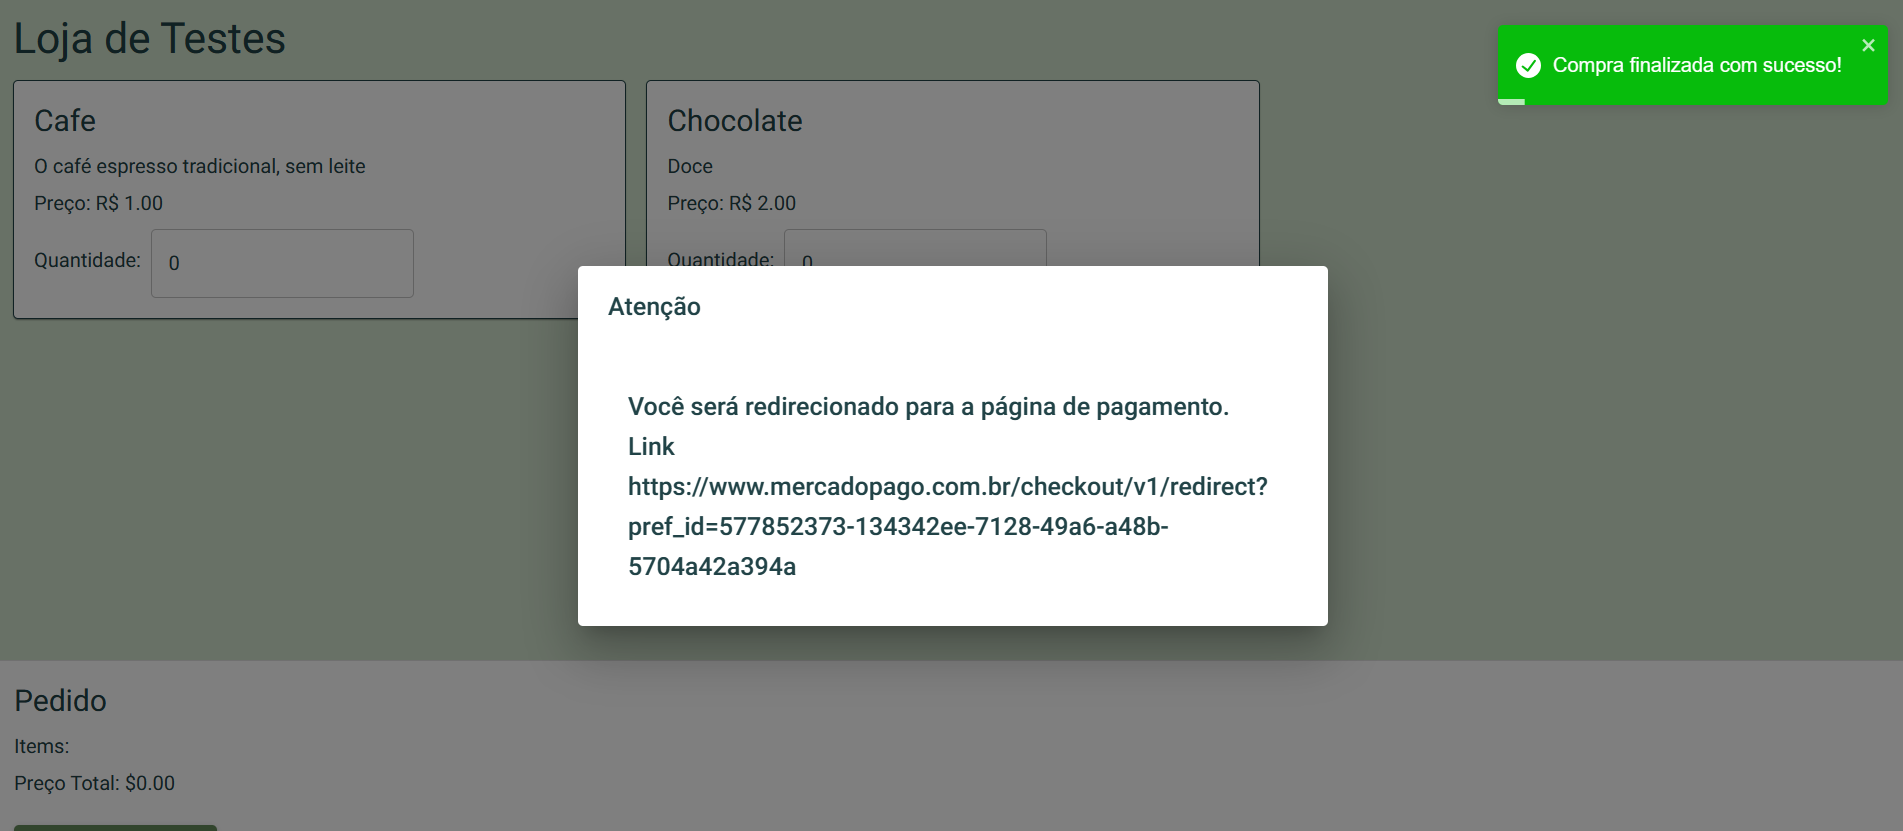
\includegraphics[width=0.8\textwidth]{figuras/avisopagamento.png}
    	\end{center}
    	\fonte{Criado pelo autor.}
    \end{figure}
    
    \item Caso o dispositivo do usuário permita, ele será redirecionado a página de pagamento. Caso contrário, ele pode pagar usando o link presente na mensagem. A página de pagamento é demonstrada na Figura \ref{fig:pagar}, nela o usuário pode selecionar o método de pagamento de sua preferência. O processo é garantido através da integração com o Mercado Pago.
    
    \begin{figure}
    	\caption{\label{fig:pagar}Tela de pagamento.}
    	\begin{center}
    		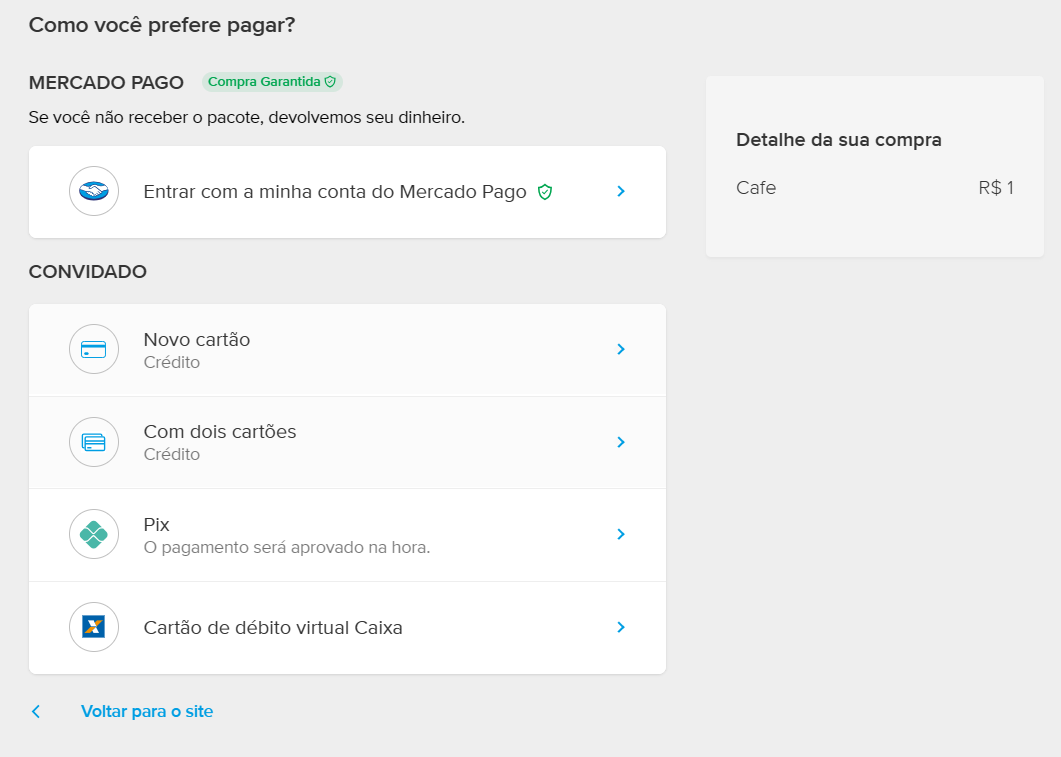
\includegraphics[width=0.8\textwidth]{figuras/pagamento.png}
    	\end{center}
    	\fonte{Criado pelo autor.}
    \end{figure}

    \item Quando o pagamento é recebido e confirmado pela API, o status do pedido é atualizado no sistema, ficando visível na interface. Caso seja um ponto de vendas do tipo automático, uma mensagem com o id do item adquirido é enviada no \textit{socket} do ponto de vendas.

    \item Caso o ponto de vendas tenha um agente de distribuição conectado, o pedido será entregue por este de forma automática. Caso o ponto de vendas seja do tipo manual, um responsável pelo ponto de vendas deve acompanhar os pedidos na interface do sistema, e realizar as entregas. Neste exemplo, o agente de distribuição é um NodeMCU que está programado para acender um led, de forma a demonstrar o recebimento do pedido, como exibido na Figura \ref{fig:nodeled}.

    \begin{figure}
    	\caption{\label{fig:nodeled}NodeMCU ao identificar ID esperado no socket.}
    	\begin{center}
    		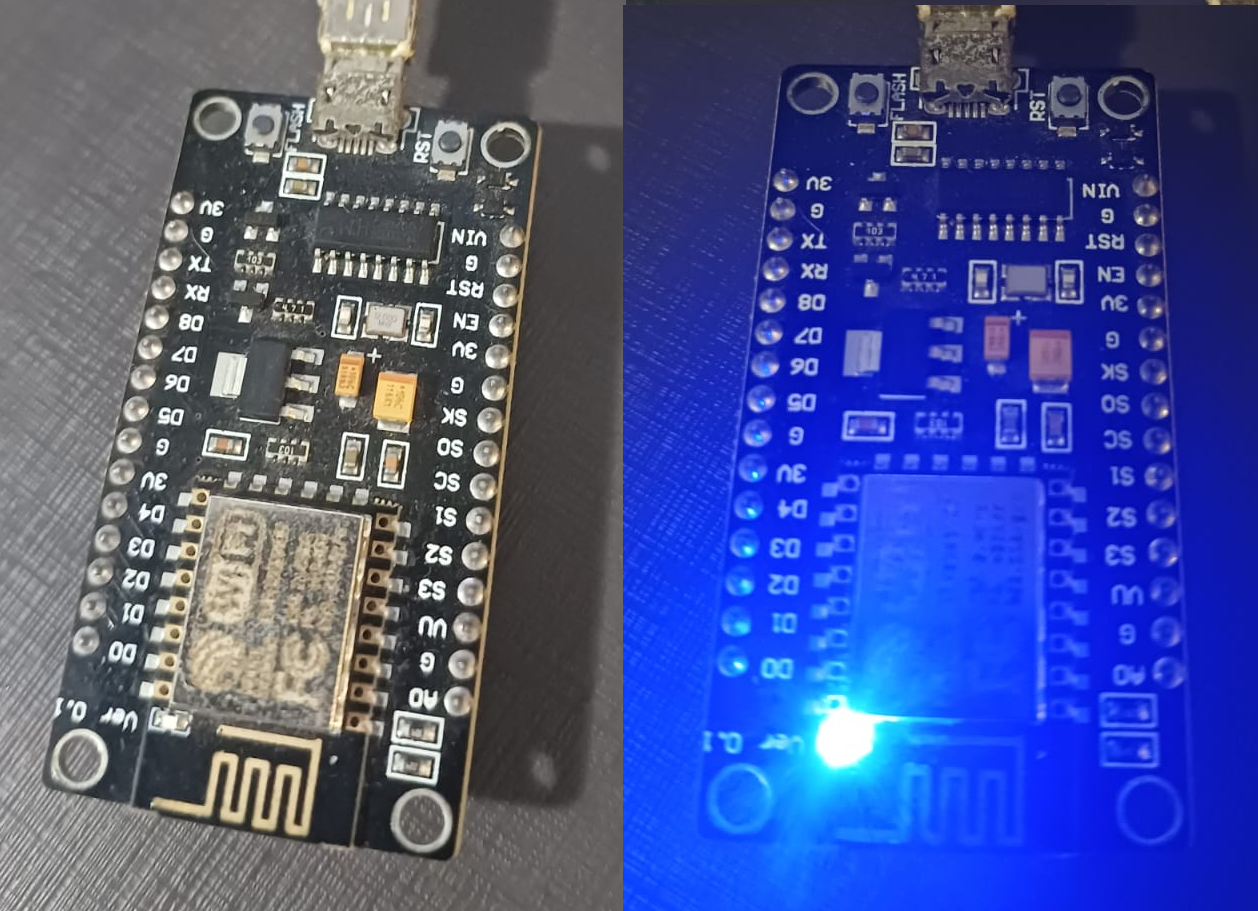
\includegraphics[width=0.5\textwidth]{figuras/nodemcunotification.png}
    	\end{center}
    	\fonte{Criado pelo autor.}
    \end{figure}
    
\end{itemize}

\section{Hospedagem e custos}\label{cap:host}

O sistema foi implantado em um ambiente de produção utilizando serviços de hospedagem em nuvem. A aplicação NextJS foi hospedada na plataforma Vercel\footnote{\url{https://vercel.com/}}. O servidor de sockets foi hospedado na plataforma Railway\footnote{\url{https://railway.app/}}. O banco de dados foi hospedado na plataforma ElephantSQL\footnote{\url{https://www.elephantsql.com/}}. A implantação foi realizada sem maiores problemas e o sistema está disponível e funcionando como o esperado. A Tabela \ref{tab:Tab_1} exibe algumas faixas de precificação para os serviços utilizados. No momento o sistema opera com os planos gratuitos.

\begin{table}[htb]
	\ABNTEXfontereduzida
	\caption{\label{tab:Tab_1}Preços dos planos de hospedagem em nuvem.}
 \begin{center}
	\begin{tabular}{@{}p{2.0cm}p{1.5cm}p{3.0cm}p{3.5cm}@{}}
		\toprule
		\textbf{Plataforma} & \textbf{Plano} & \textbf{Preço} & \textbf{Limites} \\ \midrule
		Vercel & Hobby & \ Gratuito & Projetos pessoais ou não comerciais. Deploy a partir do CLI ou integrações git. HTTPS/SSL automático. \\
		Vercel & Pro & \$20 por membro da equipe por mês. & 1TB de banda. 1000 GB/horas de execução. \\
		Vercel & Enterprise & Personalizado. & Infraestrutura de build isolada, em hardware melhor, sem filas. \\
		Railway & Starter & Gratuito & \$5.00 em créditos de recursos todos os meses com tempo de execução de 500 horas. \\
		Railway & Hobby & \$10 em créditos por mês & 8 GB de RAM / 8 vCPU por serviço \\
		Railway & Pro & \$20 por mês & Acesso compartilhado ao espaço de trabalho para equipes. \\
		Railway & Enterprise & Personalizado & Personalizado \\
		ElephantSQL & Tiny & Gratuito & 20 MB, 5 conexões concorrentes \\
		ElephantSQL & Simple & \$5 por mês & 500 MB, 10 conexões concorrentes \\
            ElephantSQL & Enormous & \$199 por mês & 250 GB, centenas de conexões concorrentes \\
  \bottomrule
	\end{tabular}
 \end{center}
	\fonte{Sites das respectivas plataformas.}
\end{table}

A hospedagem em nuvem permite a escalabilidade do sistema, o que significa que é possível aumentar a capacidade do sistema de acordo com a demanda, sem a necessidade de investimentos em infraestrutura própria.

\section{Considerações finais} \label{cap:final}

Os resultados obtidos a partir da implementação do sistema são satisfatórios e atendem aos objetivos estabelecidos neste trabalho. O sistema desenvolvido é funcional, seguro e escalável, atendendo às necessidades. As tecnologias utilizadas mostraram-se adequadas para o desenvolvimento do sistema para automação de pagamentos e para a integração de um agente de distribuição exemplificado pelo NodeMCU com a aplicação web.

